\section{Introduction}\label{sec:intro}

\subsection{Test DRP on a 3\% subset of real HSC data}

In preparation for DRP (Data Release Processing), a set of
some 17K exposures from the HSC PDR2 dataset were pushed through
a current version of the DRP pipelines.

These exposures are then coadded into 710 tracts, including about 671
WIDE tracts of repeated depth a few in grizy bands, and 39 DEEP+UDEEP with
up to 426 overlapping exposures in some bands in some UDEEP tracts.

These 17K exposures along with the coadd tracts and other
outputs generated, represent approximately 3\% of the first 
years' Rubin DR1 dataset.

 \begin{figure}
 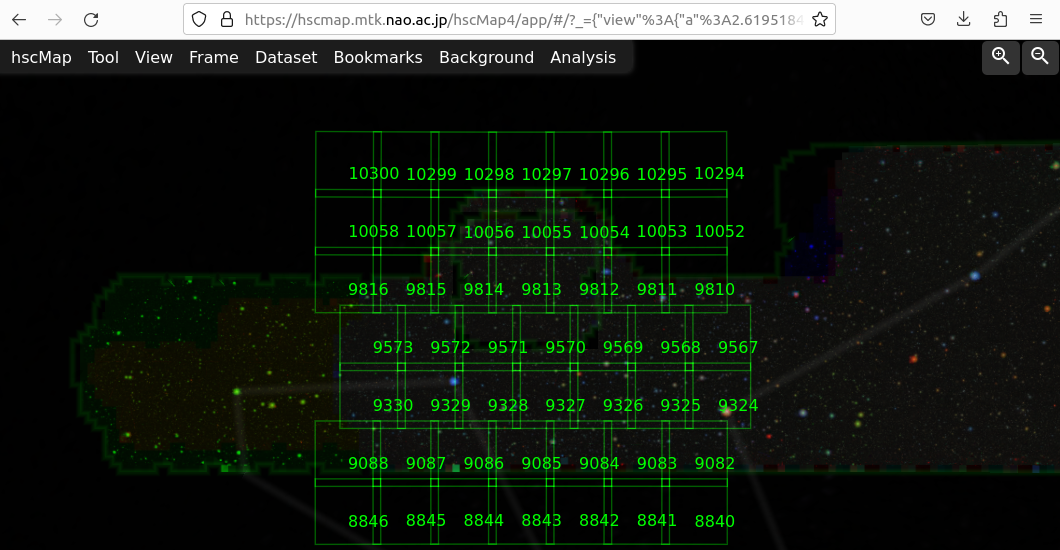
\includegraphics[width=0.9\textwidth]{hscmaptractcosmos.png}
         \caption{PDR2 close up with tract numbers.  \label{fig:hscmaptract}}
 \end{figure}



\subsection{PDR processing and instruments: HSC vs. LSSTCam}

Each detector is a 2K x 4K pixel CCD image, of size about 57MB.
There are 103 science quality CCDs/exposure.  Detector 9 is masked due
to known quality issues and ccds 104-112 are not on-sky science chips in
the HSC mosaic.

The sky is divided into 'tracts' and subdivided into 'patches',
as defined by skymap (hsc\_rings\_v1) which maps tract number to a
square region in (RA,DEC) coordinates.

For HSC, each tract covers about 2.6 sq degrees on the sky and is
subdivided into 81 patches on a $9 \times 9$ grid.


In contrast, the full LSSTCam has 4K x 4K pixel CCDs, there are 
189 science CCDs each about 100 MB in size.  Furthermore each tract 
on the sky is divided into a $7\times 7$ grid patches.

For purposes of this exercise, the calibration exposures (
flat fields in each band, biases, non-linearity maps, sky pupil per 
band and bad pixel gain and full well maps per detector) are all
taken as given 'ancillary' inputs, pre-constructed and outside the
scope of this campaign.

For DP1, DP2 and DR1 all good visits obtained to over a certain time
interval, six months to one year in length are gathered at the
start of the DRP.  All are processed through step1 (Instrument Signature
Reduction (ISR), image and PSF characterization, source detection and 
measurement), step2a (combine gather source tables), and step2b (perform 
astrometric calibration with a 2MASS or eventually Gaia reference catalog,
extract calibration star catalogs) 
at multiple processing sites if available.  Each visit may be processed
independently and in parallel.

For the PDR2 HSC exercise, multi-site was not yet up, and so all processing
was done at one site (the USDF).

Following step2b, the extracted, (and relatively small),
calibration star catalogs are gathered together over the entire campaign
footprint and are used in step2c to generate a single Forward 
Global Calibration Module (FGCM) photometric solution with zeropoints for
each exposure processed.

These astrometric solutions and photometric zeropoints from steps 2b and 2c
are applied in step2d and gathered together by visit in step2e.

There may be a 'visit-veto' rejection of poor quality (i.e. bad seeing)
exposures at the end of step2e but prior to the start of step3.  A subcollection is made containing only the remaining good visits, which are used for
further processing.  For the HSC PDR2 case, about 2.5K out of 17.3K visits
were rejected leaving about 15K visits to be coadded.

Step3 of PDR processing performs coaddition, combining all calibrated 
visit images, first 'warping' them using the astrometric solution to put 
them onto common geometric footprint and then adding them weighted appropriately
by photometric flux zeropoint and noise properties.

The astrometric algorithm used for PDR2 HSC is called 'jointcal'.  This
older algorithm may be replaced by 'gbdes' in future processings, as that
algorithm accounts for 'tree rings', DCR and other subtle distortions.

Coadds for the HSC PDR2 footprint are currently done at the patch 
level, though future processings will also produce 'overlapping cell-based' 
coadds which further subdivides patches and tracts 
into regions of the sky where the PSF in each band is well-modeled as constant 
across an entire cell with no discontinuous jumps due to detector edges.
These cell-based coadds in turn allows for the accurate measurement of 
weak lensing shears of all source stacked objects when combined with
a PIFF PSF model.

Between May 2023 and (approx) Sep 2023 the HSC PDR2 was reprocessed with 
Rubin Science pipelines stack version v24.1.0, which was 
based on a weekly stack w\_2023\_7.  Some modifications or fixes to the stack
were applied during the processing, as described below.

In this document we discuss campaign management \secref{sec:management},
processing \secref{sec:processing} and quality 
assurance \secref{sec:processing} details of the HSC PDR2 reprocessing.

%5\begin{itemize}
%\item Campaign Management and communication is discussed in \secref{sec:management}
%\item An overview of the processing is given in \secref{sec:processing}
%\item Quality assurance and feedback to processing is discussed in  \secref{sec:qa}
%\end{itemize}

